\section{Analiza i specyfikacja wymagań (Bogna Lew)}\label{s:wymagania}
W niniejszej sekcji przedstawiono specyfikę wymagań funkcjonalnych, pozafunkcjonalnych oraz tych, wynikających z
głównych założeń projektu. Dodatkowo zawiera ona diagramy przypadków użycia, maszyny stanów oraz klas prototypowej gry.

\subsection{Specyfika wymagań wynikających z założeń projektu}
“Starożytni świat widzieli inaczej, mniej płasko”\cite{gbobrektvgry}. Dobrze obrazującym ówczesne postrzeganie
przestrzeni przykładem jest mapa Imperium Rzymskiego, pokazana na \ref{fig:mapaIR}. Czytanie jej dosłownie mija się z
celem. Nie są na niej zachowane ani proporcje, ani strony świata. Mimo tego, że basen Morza Śródziemnego został
ówcześnie dosyć dokładnie oddany, “nie wydaje się, aby Rzymianom współczesna kartograficzna wierność była potrzebna”\cite{gbobrektvgry}.
“Dowódcy opierali się na swojej wiedzy, wiedzy wynajętych przewodników oraz informacjach zwiadowców i tubylców”\cite{gbobrektvgry}.

\begin{figure}[htbp]
    \centering
    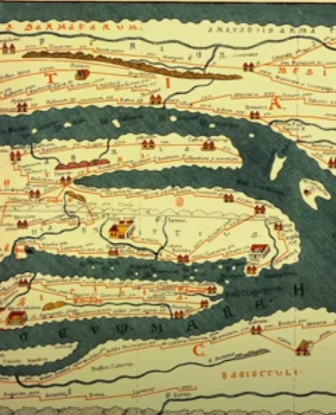
\includegraphics[width=0.5\textwidth]{images/mapaIR.png}
    \caption{Mapa basenu Morza Śródziemnego z czasów Imperium Rzymskiego}\label{fig:mapaIR}
\end{figure}

Z punktu widzenia projektu kluczowe jest jak najdokładniejsze oddanie realiów historycznych przy jednoczesnym
uwzględnieniu jakości rozgrywki gracza oraz cech charakterystycznych dla gier typu RTS. Z założeń wynika, że fabuła
gry powinna zostać osadzona w czasach sprzed wielkich odkryć geograficznych. Na tej podstawie zostały zdefiniowane
dodatkowe wymagania, które powinien spełniać prototyp:
\begin{itemize}
  \item Sposób nawigacji powinien jak najdokładniej odpowiadać temu stosowanemu w wybranej epoce;
  \item Postacie w grze powinny stylistycznie pasować do realiów historycznych;
  \item Postacie powinny posługiwać się słownictwem adekwatnym do czasów, w których osadzona jest gra;
  \item Postacie powinny jak najlepiej oddawać światopogląd w danych czasach;
  \item Oręż stosowany w grze powinien odpowiadać realiom historycznym;
  \item Budowle w grze powinny stylistycznie odpowiadać wybranej epoce;
  \item Sposób komunikacji z postaciami powinien imitować ten stosowany w danych czasach;
\end{itemize}

\subsection{Wymagania funkcjonalne}\label{ss:fun}
W przedstawionej liście zostały wymienione wymagania funkcjonalne, które powinien spełniać prototyp gry.

\begin{itemize}\label{list:fun}
  \item Zapis oraz odczyt wybranego stanu gry lokalnie na komputerze użytkownika;
  \item Uruchomienie nowej gry;
  \item Możliwość sterowania postacią gracza;
  \item Możliwość nawigacji w świecie gry;
  \item Możliwość wchodzenia w interakcję z postaciami niezależnymi;
  \item Możliwość przyjmowania zleceń od postaci niezależnych;
  \item Możliwość najmowania postaci wojowników;
  \item Możliwość wydawania komend wynajętym postaciom;
  \item Możliwość zlecania budowy;
  \item Możliwość zdobywania zasobów;
\end{itemize}

\subsection{Wymagania pozafunkcjonalne}\label{ss:nonfun}
Poniższa lista przedstawia wymagania niefunkcjonalne projektu.

\begin{itemize}\label{list:nonfun}
  \item Rozgrywka w trybie offline;
  \item Działanie na urządzeniach z systemem Windows lub Linux;
  \item Dostosowywanie rozmiaru do wielkości ekranu komputera użytkownika;
  \item Obsługa klawiatury oraz myszy;
  \item Działanie w czasie rzeczywistym;
\end{itemize}

\subsection{Diagram przypadków użycia}\label{ss:usecase}
Niniejsza sekcja przedstawia diagram przypadków użycia dla głównych funkcjonalności, które będzie zawierać prototypowa gra.
Opisuje on przewidywane usługi oferowane przez poszczególne mechaniki programu.

Jedną z głównych akcji, które gra udostępni będzie wydanie rozkazów przyjaznym jednostkom. Polegać będzie ona na poinformowaniu
wojowników przez gracza jaką czynność powinni w danym momencie wykonać. Kolejną możliwością będzie zlecenie budowy, czyli
zlecenie budowniczemu wybudowania wybranego obiektu w określonym przez gracza miejscu. Ponadto użytkownik
będzie mógł przeprowadzać rozmowy z postaciami niezależnymi. Oznacza to, że będzie mógł zainicjować z nimi dialog i
następnie kształtować jego przebieg poprzez wybieranie swojej odpowiedzi z opcji proponowanych przez grę.

\begin{figure}[!htbp]
    \centering
    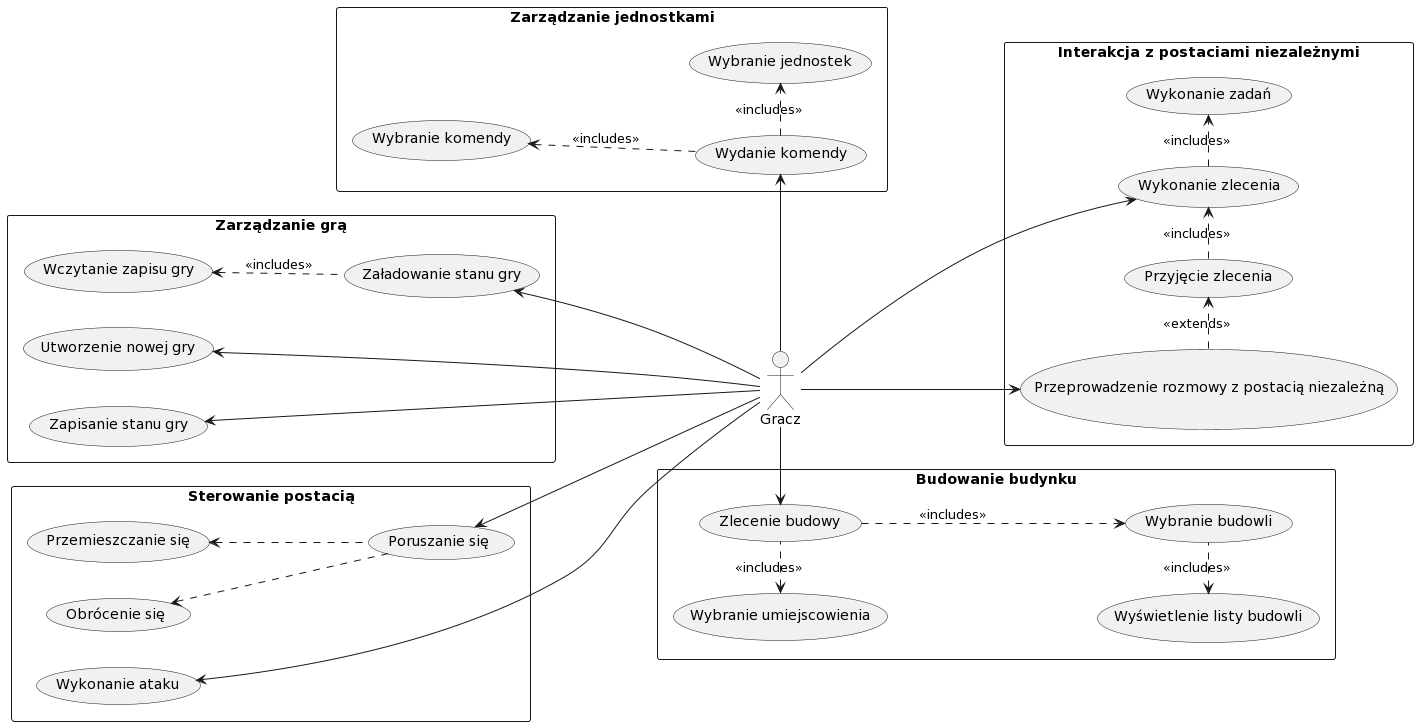
\includegraphics[width=1.0\textwidth]{images/diagrams/usecase.jpg}
    \caption{Diagram przypadków głównych mechanik gry.}\label{fig:usecases}
\end{figure}
\FloatBarrier

\subsection{Diagram stanów}\label{ss:state}
W tym podpunkcie został przedstawiony diagram stanów prototypowej gry, który ukazuje jej przewidywany sposób działania.
Prezentuje on podstawowe stany, w których może się znaleźć system gry.

Do podstawowych stanów należą "Menu główne" oraz "Rozgrywka". Pierwszy z nich oznacza, że program został uruchomiony, a
gracz wyświetla panel główny. Z tego stanu możliwe jest przejście do stanów "Odczytanie stanu gry" bądź "Utworzenie
nowej gry", które to powodują rozpoczęcie gry z zapisu lub od początku.

Stan "Rozgrywka" jest stanem złożonym i określa, że gra została rozpoczęta. W jego skład wchodzą przede wszystkim takie
stany, jak "Interakcja z postacią niezależną", w którym program się znajdzie, gdy gracz rozpocznie dialog z postacią w grze,
czy "Zarządzanie jednostkami", który to oznacza, że użytkownik wydaje rozkazy swoim wojownikom.

Diagram stanów został przedstawiony na rysunku \ref{fig:states}.

\begin{figure}[!htbp]
    \centering
    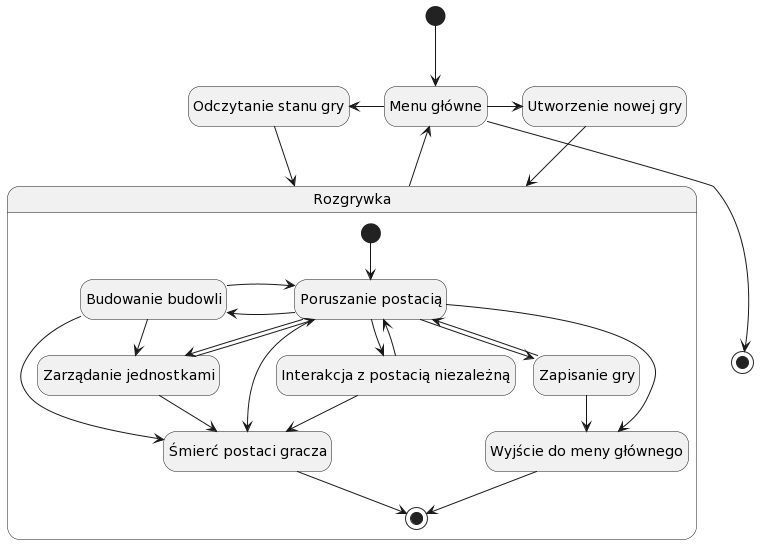
\includegraphics[width=1.0\textwidth]{images/diagrams/state.jpg}
    \caption{Diagram stanów gry.}\label{fig:states}
\end{figure}
\FloatBarrier

\subsection{Diagram klas}\label{ss:class}
W tej sekcji został pokazany uproszczony diagram klas (rys. \ref{fig:classes}), przedstawiający główne elementy gry.
Obrazuje podstawową strukturę tworzonego systemu oraz zależności pomiędzy poszczególnymi komponentami.

Do najważniejszych klas należą "Interfejs użytkownika", "Mechanizm interakcji z postaciami", "Mechanizm zarządzania
jednostkami" oraz "Mechanizm budowania". Obrazują one podstawowe komponenty gry, których głównym zadaniem jest zarządzanie
poszczególnymi mechanikami. "Interfejs użytkownika" jest odpowiedzialny za interakcję z graczem oraz pomaganie mu w
trakcie rozgrywki. Pozostałe trzy kolejno pozwalają graczowi na prowadzenie dialogów z postaciami
niezależnymi, wydawanie komend jego zaprzyjaźnionym jednostkom oraz budowanie obiektów.
\begin{figure}[!htbp]
    \centering
    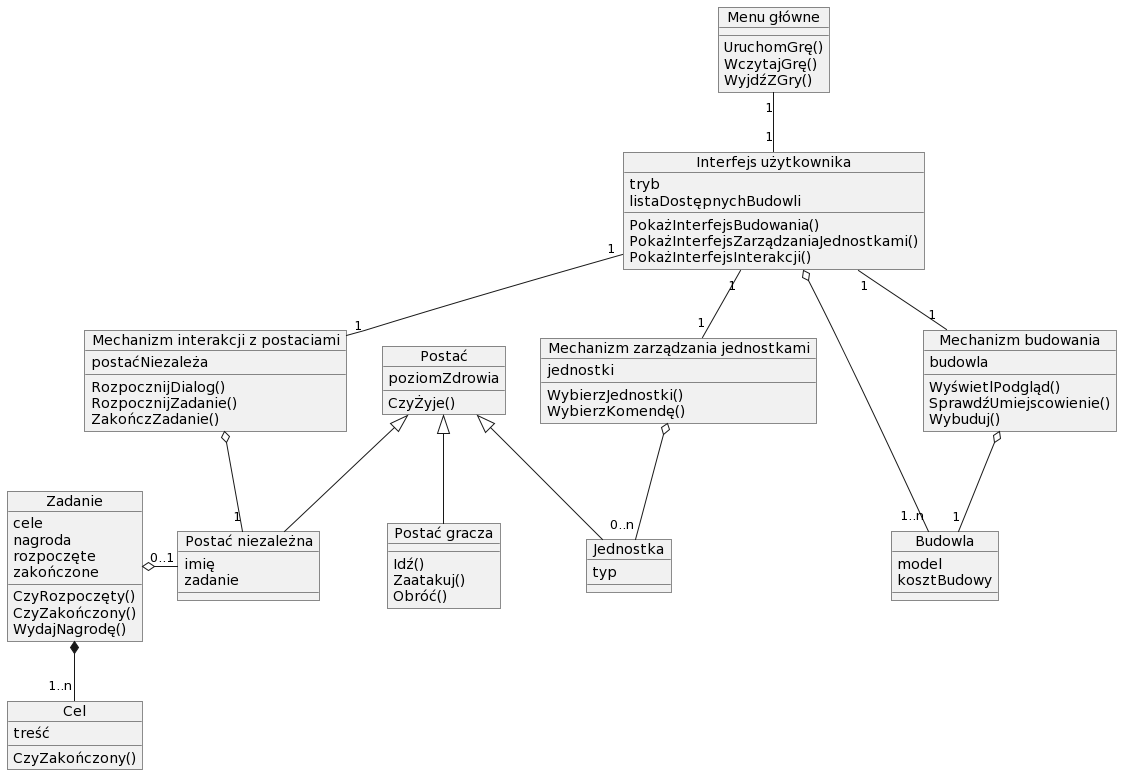
\includegraphics[width=1.0\textwidth]{images/diagrams/class.jpg}
    \caption{Diagram klas gry.}\label{fig:classes}
\end{figure}